
\setchapterimage[6cm]{intro/bucketsAndBalls/Basketball.png}
\setchapterpreamble[u]{\margintoc}
\chapter{Buckets and Balls\protect\footnotemark}
\labch{ch-bb}

\footnotetext{A basketball ball about to fall through the hoop. Author: \href{https://commons.wikimedia.org/wiki/File:2011-06-07_Basketball_in_hoop_still_shot.jpg}{Ildar Sagdejev / 2011 / GNU General Public License}.}
\footnotetext{This chapter is based on the article~\cite{bucketsAndBalls}.}

The notion of ``Linked Data`` is still a misunderstood and underestimated concept. Perhaps this data seems too complex.
Let's try to figure it out. Let's start with variables.

\begin{marginfigure}[-1.5cm]
	{
		\setlength{\fboxsep}{0pt}%
		\setlength{\fboxrule}{1pt}%
		\fcolorbox{gray}{gray}{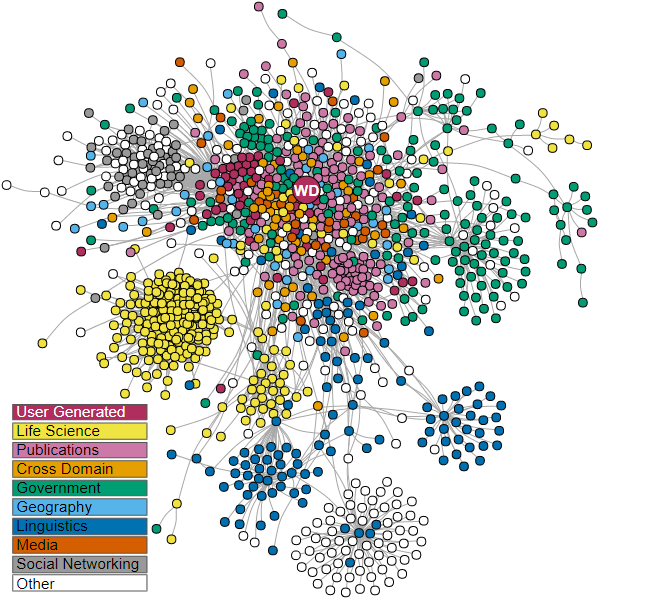
\includegraphics{./intro/bucketsAndBalls/Wikidata_in_linked_open_data.png}}
	}
    \caption[Wikidata in the Linked Open Data Cloud]{Wikidata in the Linked Open Data Cloud. Databases indicated as circles (with wikidata indicated as \textit{WD}), with grey lines linking databases in the network if their data is aligned. See the wikipedia article: \href{https://en.wikipedia.org/wiki/Linked_data}{Linked data}. Wikimedia Commons / \href{https://commons.wikimedia.org/wiki/File:Wikidata_in_the_Linked_Open_Data_cloud_2020-08-20.svg}{Thomas Shafee}}
	\label{fig:Wikidata_in_linked_open_data}
\end{marginfigure}

What is a variable in SPARQL? Let it be something that needs to be filled with something. But how to imagine this ``that``? Something abstract is easier to imagine if connected with something physical and concrete. It is difficult to imagine the time, but as soon as we imagine a clock with hands, it becomes easier. We cannot imagine furniture in general, but everyone can imagine a chair. 

Another difficulty lies in formulating the query in SPARQL language. Although working with SPARQL helps to understand how the knowledge graph\sidenote[][*6]{\index{Computer Science!Knowledge Graph} Knowledge graph is a knowledge base that uses a graph-structured data model to integrate data. Knowledge graphs are often used to store interlinked descriptions of entities~--- objects, events, situations or abstract concepts works. Next, a knowledge graph will be built (Pic.~\ref{fig:Graph_pattern_in_basket_and_balls_notation}).}, the SPARQL query does not look like it. It is like with symbols in mathematics. ``5~doesn`t look like five, while ||||| is five''.

So how do you solve the problem of defining a variable and formulating a SPARQL query?

Imagine each SPARQL query as a graph of baskets and balls related to each other. 

Let variables be something that needs to be filled, but now a variable is an abstract concept. We need a physical container to fill it with things. We need baskets. And things are like balls. So let's imagine the execution of a query as filling baskets with balls.

Then the process of filling the graph with balls will look like in Pic.~\ref{fig:Query_as_filling_buckets_with_balls}. A bucket \textbf{?A} should be filled with those balls which have a relation \textbf{R} to ball \textbf{B}.

\begin{marginfigure}
	{
		\setlength{\fboxsep}{0pt}%
		\setlength{\fboxrule}{1pt}%
		\fcolorbox{gray}{gray}{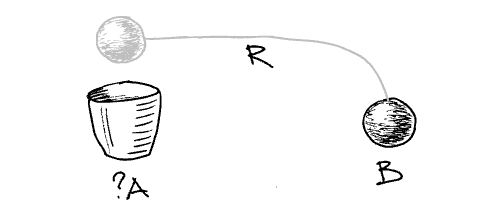
\includegraphics{./intro/bucketsAndBalls/graphPattern.PNG}}
	}
    \caption{Sample graph of filling baskets with balls.}
	\label{fig:Query_as_filling_buckets_with_balls}
\end{marginfigure}

The drawing will be clearer if we simplify it and draw a straight line (Pic.~\ref{fig:Graph_pattern_in_basket_and_balls_notation}). This is a graph pattern in Buckets`n`Balls notation. The direction of the relation R is not shown but it`s always from left to right.

\newpage
The process of writing and running a SPARQL query would then go through the following steps:
\begin{enumerate}
    \item Select your buckets (in them you are going to gather the balls you want).
    \item Compose your conditions as a graph of buckets and balls.
    \item Run your query to fill your buckets with balls.
\end{enumerate}

\begin{marginfigure}[-3cm]
	{
		\setlength{\fboxsep}{0pt}%
		\setlength{\fboxrule}{1pt}%
		\fcolorbox{gray}{gray}{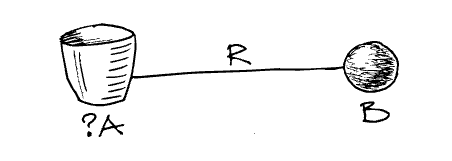
\includegraphics{./intro/bucketsAndBalls/graphPatternBucketsBalls.PNG}}
	}
    \caption{Graph pattern in Buckets`n`Balls notation.}
	\label{fig:Graph_pattern_in_basket_and_balls_notation}
\end{marginfigure}

Now we will write a request to, for example, get all the heads of the regions of Russia by following these steps:

\begin{enumerate}
    \item Let's take two baskets, one for regions and one for heads.
    \item We will tie the basket for regions to the ball ``region of Russia`` with the relation ``instance`` (instance of). Then from the set of balls~--- objects of Wikidata~--- only those balls that are the region of Russia will fall into this basket. The basket for regions is connected to the basket ``head` by the relation ``has a head``, in our case it will be the governor or the head of the region.
\end{enumerate}

Let`s make the request more interesting and add another basket for photos of governors. Now the query in the notation ``Buckets`n`Balls`` will be as in Pic.~\ref{fig:Query_in_basket_and_balls_notation}.

\begin{figure}[h!]
    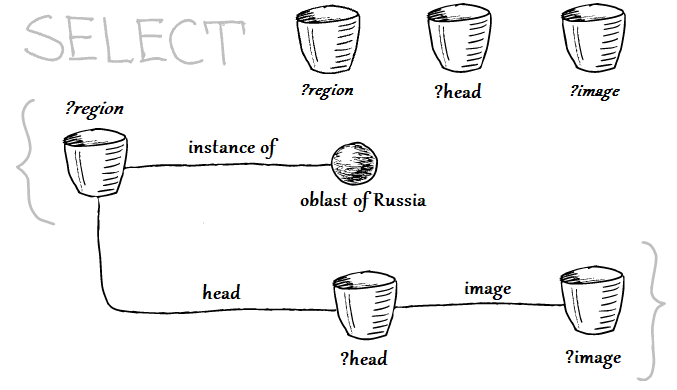
\includegraphics{./intro/bucketsAndBalls/Query_in_basket_and_balls_notation.PNG}
    \caption{Query in the notation ``Buckets`n`Balls`` to fill the baskets with ``region`` balls ``region of Russia``, ``head``~--- governors or heads of the region, ``image``~--- their photos.}
	\label{fig:Query_in_basket_and_balls_notation}
\end{figure}

After running the request (Pic.~\ref{fig:Query_in_basket_and_balls_notation}) our baskets will look like in Pic.~\ref{fig:3_buckets_region_head_image}.

\begin{marginfigure}
	{
		\setlength{\fboxsep}{0pt}%
		\setlength{\fboxrule}{1pt}%
		\fcolorbox{gray}{gray}{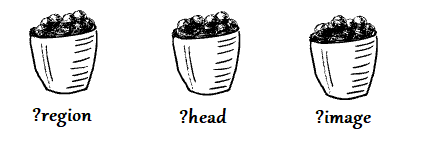
\includegraphics{./intro/bucketsAndBalls/3_buckets_region_head_image.PNG}}
	}
    \caption{Baskets after running the request in Pic.~\ref{fig:Query_in_basket_and_balls_notation}. \textit{?region} these are the regions of Russia, \textit{?head} these are the heads, \textit{?image}~--- these are photos of heads.}
	\label{fig:3_buckets_region_head_image}
\end{marginfigure}

Now let`s go to the service \href{https://query.wikidata.org/}{Wikidata Query Service} (next WDQS\sidenote[][]{See the explanations about WDQS at p.~\pageref{ch:review-wd}.}) and we will write this query in SPARQL. First, we will select and name the baskets to fill as follows:

\begin{lstlisting}[ language=SPARQL, numbers=none]
SELECT DISTINCT ?region ?head ?image
\end{lstlisting}

Next, we will write the conditions for matching balls to baskets. All conditions in SPARQL should be enclosed in curly brackets, as in Pic.~\ref{fig:Query_in_basket_and_balls_notation}.

Whenever we need a specific relation or ball, we need to use their identifiers. Wikidata makes it easy to find an identifier and suggest it when you select a relation (property) or ball (object) by its name (label). To indicate relationships in the Wikidata knowledge graph, we use the \textit{wdt:} prefix, and for objects (our balls)~--- the \textit{wd:} prefix. 

Following our notation (Pic.~\ref{fig:Query_in_basket_and_balls_notation}), we will write conditions for filling the first basket \textit{?region}, then we will write the first relation. Since the common part of direct relationship identifiers is wdt, we write \textit{wdt:} and then, in the WDQS service, press Ctrl+Space to start the Wikidata hint or autocomplete service (Pic.~\ref{fig:WDQS_popup_instance_of}). 

\begin{marginfigure}[-2cm]
	{
		\setlength{\fboxsep}{0pt}%
		\setlength{\fboxrule}{1pt}%
		\fcolorbox{gray}{gray}{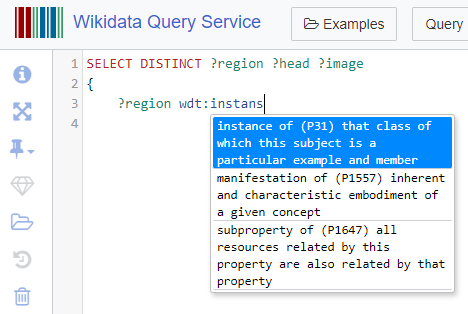
\includegraphics{./intro/bucketsAndBalls/WDQS_popup_instance_of.PNG}}
	}
    \caption{Using the Ctrl+Space command, the drop-down context menu for autofill Wikidata properties opened.}
	\label{fig:WDQS_popup_instance_of}
\end{marginfigure}

After that, we will reproduce the model from Pic.~\ref{fig:Query_in_basket_and_balls_notation} in a real SPARQL query.

Usually, when writing a SPARQL query, it is presented as a table with three columns: subject, predicate, object, or in the Wikidata language~--- object, property, value.

Perhaps a beginner programmer will find it easier to master SPARQL if at least your first queries resemble a graph. Let's try to take the graph in Pic.~\ref{fig:Query_in_basket_and_balls_notation} and write a SPARQL query in the most similar way (listing~\ref{lst:linkRegionsOfHeads}).

\begin{lstlisting}[ language=SPARQL, numbers=none, caption={List of heads of regions of Russia with photos. 
                    Received 44 references to the regions of Russia and their heads of government. 
                    Link to SPARQL query: \href{https://w.wiki/4NVc}{https://w.wiki/4NVc}},
                    label=lst:linkRegionsOfHeads]
SELECT DISTINCT ?region ?head ?image
{
    ?region wdt:P31 wd:Q835714; # oblast of Russia
            wdt:P6  ?head. # heads of government
    ?head  wdt:P18 ?image. # images of heads of government
}
\end{lstlisting}

Now look at how this request looks in the WDQS service, and run it. Then click on the eye icon on the left and select \textit{``image grid``} (Pic.~\ref{fig:WDQS_drop_down_result_type}) to view the results as an image grid.

\begin{marginfigure}[-1cm]
	{
		\setlength{\fboxsep}{0pt}%
		\setlength{\fboxrule}{1pt}%
		\fcolorbox{gray}{gray}{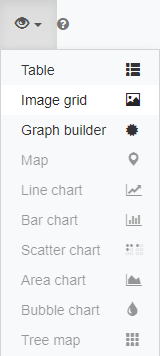
\includegraphics[width=0.5\linewidth]{./intro/bucketsAndBalls/WDQS_drop_down_result_type.PNG}}
	}
    \caption{Selecting the display of results as \textit{``image grid``}.}
	\label{fig:WDQS_drop_down_result_type}
\end{marginfigure}

This is not bad for the first result, but now under each photo we see only the IDs of people and areas. If we click on the ID hyperlink, we will get a lot of information about this object. But it would be clearer to specify the names of people and the names of areas (labels) in addition to identifiers as a result of the request. It`s like putting labels on our baskets (Pic.~\ref{fig:Query_in_basket_and_balls_notation_with_ids}).

\begin{figure}[h!]
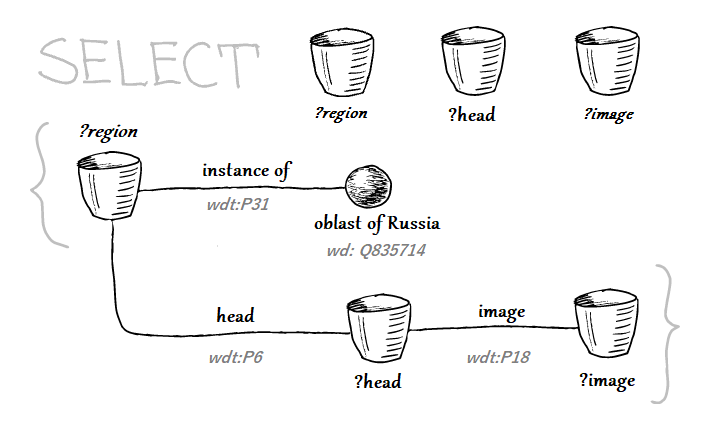
\includegraphics{./intro/bucketsAndBalls/Query_in_basket_and_balls_notation_with_ids.png}
\caption{A query in the notation ``Buckets`n`Balls`` with the numbers of properties and objects of Wikidata.}
\label{fig:Query_in_basket_and_balls_notation_with_ids}
\end{figure}

A label is something that every ball has, that is, a Wikidata object. A label is a name that allows you to distinguish objects from each other. Wikidata has a service that simplifies the output of labels on request. To do this, just add the word \textit{"Label"} to the end of the variable name and call the desired service. To call this service, type Ctrl + space on a new line inside curly brackets and when you start writing the word \textit{"Label"}, then a line with this service will be added\sidenote[][]{An example of calling this service is provided in listing ~\ref{lst:regionsOfHeads}}. By default, you get a hint with the interface language and English as an alternative if the label is not available in the language of the selected Wikidata interface.

Wikidata is full of such wonderful services, and for the final request we will use another one. To get the result immediately in the form of a set of photos of the heads of the regions, without additional clicking on the eye icon, place the following construction for WDQS somewhere in your request:
\begin{lstlisting}[ language=SPARQL, numbers=none ]
#defaultView:ImageGrid
\end{lstlisting}

In fact, not everything needs to be written manually. When you start typing, the autofill service will offer options.

Our last request is presented on the listing ~\ref{lst:regionsOfHeads}. A fragment of the result of its running is shown in Pic.~\ref{fig:Result_of_the_request}.

\begin{lstlisting}[ language=SPARQL, caption={List of heads of regions of Russia. 
                    Received 44 references to the regions of Russia and their heads of government. 
                    Link to SPARQL query: \href{https://w.wiki/4bGf}{https://w.wiki/4bGf}},
                    label=lst:regionsOfHeads, ]
# List of regions of the Russia and images of heads of government
#defaultView:ImageGrid
SELECT DISTINCT ?region ?regionLabel ?head ?headLabel ?image
{
  ?region wdt:P31 wd:Q835714; # ?region is Oblast of Russia
          wdt:P6  ?head.      #         has head of government
  ?head  wdt:P18 ?image.      # head has image
  SERVICE wikibase:label {bd:serviceParam wikibase:language "en"} 
}
\end{lstlisting}

\begin{figure}[h!]
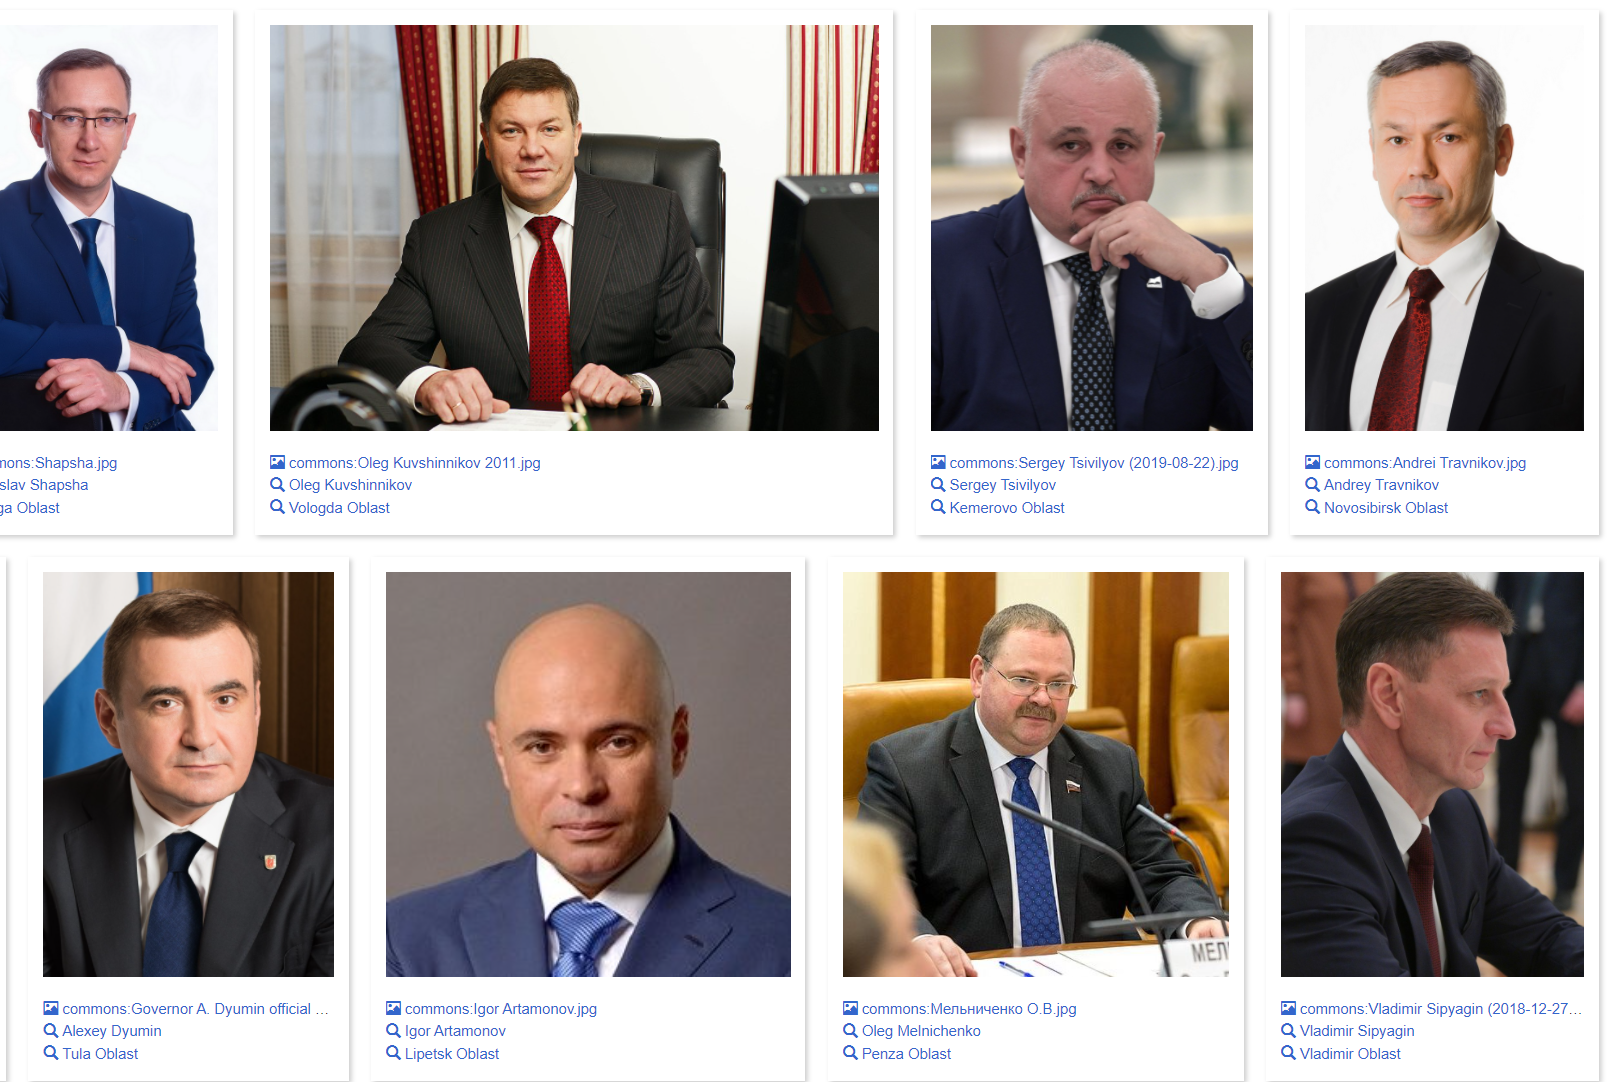
\includegraphics{./intro/bucketsAndBalls/result_of_request_for_photos_of_heads_of_government_en.png}
\caption{The result of the request in the form of a grid of images.}
\label{fig:Result_of_the_request}
\end{figure}

Thinking of SPARQL queries as linked baskets and balls can be helpful, at least at the beginning of the development of Wikidata. And, of course, every metaphor has its limitations. For example, you can't put the same ball in two different real baskets, but in these virtual~--- you can. <<Baskets and balls>> can be useful to climb to the height of the abstraction of Wikidata.
